\documentclass[a4paper]{article}
\usepackage[english]{babel} % ???????????
\usepackage[margin=20mm]{geometry}
\renewcommand{\baselinestretch}{1.5} 
\usepackage[utf8]{inputenc}
\usepackage{amsmath}
\usepackage{physics}
\usepackage{stackengine}
\usepackage{array, makecell} 
\usepackage[dvips]{hyperref} 
\usepackage{lscape}
\usepackage[toc,page]{appendix}
\usepackage{float}
\usepackage{cleveref}
\usepackage{thm-autoref}
\usepackage{placeins}
\usepackage{multirow}
\usepackage{amsfonts}
\usepackage{amssymb}
\usepackage{lipsum}
\usepackage{authblk}
\usepackage{graphicx}
\usepackage{longtable}
\usepackage{subfig,subcaption,siunitx,booktabs}
\usepackage{tabularx,siunitx}
\usepackage[dvipsnames]{xcolor}
\usepackage[linesnumbered, ruled, vlined]{algorithm2e}
\usepackage{lscape}
\usepackage{amsthm} % ?????????

\newtheorem{thm}{Theorem}
\newtheorem{lemma}{Lemma}
\newtheorem{prop}{Proposition}


\newtheorem{cor}{Corollary}[thm]
\newtheorem{defn}{Definition}
\newtheorem{conj}{Conjecture}
\newtheorem{con}{Condition}
\newtheorem{exmp}{Example}
\newtheorem{rem}{Remark}
\newtheorem{note}{Note}
\newtheorem{assu}{Assumption}

\DeclareMathOperator{\diag}{diag}

\crefname{lemma}{lemma}{lemma}
\usepackage{verbatim}
\usepackage{csquotes}
\usepackage{natbib}
\hypersetup{
colorlinks,
linktoc=all,
linktocpage=true,
citecolor=blue,
breaklinks=true,
filecolor=blue,
linkcolor=red,
urlcolor=blue,
linktocpage=true
}
\providecommand{\keywords}[1]
{
\small
\textbf{\textit{Keywords---}} #1
}

\sloppy 
\begin{document}
\title{Augment Large Covariance Matrix Estimation With Auxiliary Network Information \thanks{The authors would like to thank Xiaohong Chen, Hashem Pesaran, Cheng Hsiao, Harrison Zhou, Seok Young Hong, Jeroen Dalderop for their useful comments.}}
    \author[]{Shuyi Ge\thanks{School of Finance, University of Nankai. Author email:sg751@cam.ac.uk}}
    \author[]{Shaoran Li\thanks{School of Economics, Peking University. Author email:sl736@cam.ac.uk}}
    \author[]{Oliver Linton\thanks{Faculty of Economics, University of Cambridge. Author email:obl20@cam.ac.uk}}
    \author[]{Weiguang Liu\thanks{Faculty of Economics, University of Cambridge. Author email:wl342@cam.ac.uk}}
    \author[]{Xiang Lu\thanks{School of Electronics Engineering and Computer Science, Peking University. Author email:1900012773@pku.edu.cn}}
    \affil[]{}
    \maketitle
\begin{abstract}
In this paper, we propose two novel frameworks to incorporate auxiliary information about connectivity among entities (i.e., network information) into the estimation of large covariance matrices. The current literature either completely ignores this kind of network information (e.g., thresholding and shrinkage) or utilizes some simple network structure under very restrictive settings (e.g., banding). In the era of big data, we can easily get access to auxiliary information about the complex connectivity structure among entities. Depending on the features of the auxiliary network information at hand and the structure of the covariance matrix, we provide two different frameworks correspondingly\textemdash the Network Guided Thresholding and the Network Guided Banding. We show that both Network Guided estimators have optimal convergence rates over a larger class of sparse covariance matrix. Simulation studies demonstrate that they generally outperform other pure statistical methods, especially when the true covariance matrix is sparse, and the auxiliary network contains genuine information. Empirically, we apply our method to the estimation of the covariance matrix of asset returns to attain the global minimum variance (GMV) portfolio.  
\bigskip

Keywords: Big data; network; large covariance matrix; thresholding; banding.

JEL Classification: 
\end{abstract} \hspace{10pt}
\pagebreak
\normalsize
\section{Introduction}
Covariance matrix estimation is an important problem in statistics
and econometrics. When the dimensionality $N$ of the random vector $\boldsymbol{X}_t=(X_{1t},\dots,X_{Nt})^{\intercal}$ under inspection is large, estimating its covariance matrix is challenging. It is well known that the sample covariance matrix is ill-conditioned when the dimension exceeds the sample size. In that case, some structures need to be imposed on the covariance matrix, and regularization techniques need to be applied for consistent estimation. 

In the era of big data, we are gaining access to more and more auxiliary information apart from the observations of $\{\boldsymbol{X}_t\}_{t=1}^T$, which could potentially help us learn about the underlying structure of the covariance matrix (i.e., connectivity among entities). Consider the case of equity return covariance. \cite{israelsen2016does} finds that stocks covered by similar sets of analysts co-move a lot. \cite{ge2022news} find that stocks co-mentioned in business news exhibit excess co-movement beyond risk factors. Apply textual analysis to firms' 10-K reports, \cite{hoberg2016text} define peer groups within which firms are fundamentally similar. All these aforementioned auxiliary network information could help us to learn about the connectivity among the stocks. However, the current literature either completely ignores this kind of auxiliary information or uses part of them under some very restrictive settings. 

In this paper, we incorporate auxiliary information about connectivity among entities (i.e., network information) into the estimation of large covariance matrices. Depending on the features of the auxiliary network information at hand and the structure of the covariance matrix, we provide separate avenues for application and derive their theories accordingly. 

The first method we propose is called Network Guided Thresholding. The method is applicable when auxiliary information identifies the location of “significant” elements in the covariance matrix while staying silent about the relative importance of neighbors for each node. For instance, industry information is a good example of such auxiliary information as it implies a block-diagonal network where every node is equal within an industry. The original series of thresholding methods (\cite{bickel2008CovarianceRegularization}, \cite{cai2011adaptive}, \cite{fan2013large}) keep the “significant” elements in the sample covariance and shrink the rest based on statistical information only under the assumption of sparsity (or conditional sparsity). These thresholding estimators require no knowledge about the location information. We, on the other hand, utilize auxiliary network information to identify the location of these “significant” elements. We keep the “significant” elements in the sample covariance and then apply generalized thresholding to the rest. The work closest to this method is \cite{fan2016incorporating}, where the authors apply location-based thresholding utilizing sector information. However, the factor model residual correlation structure is not as simple as a block diagonal assumed by \cite{fan2016incorporating}, and our method accommodates more complex structures. We derive the theoretical properties of the Network Guided Thresholding estimator. Compared with \cite{bickel2008CovarianceRegularization}, we consider a larger class of sparse covariance matrices as we distinguish "large" and "small" elements using the auxiliary information and we quantify their behaviors separately.
We show the consistency of the estimator in the operator norm as $(log N)/T\to 0$, uniformly over the class of matrices that satisfy our sparsity condition. And we also show that the Network Guided Thresholding estimator achieves optimal rate as in \cite{bickel2008CovarianceRegularization} over a larger parameter space. Simulation results show that its finite sample performance is better than all other pure statistical methods as long as the auxiliary network information is decent (not too much type I and type II errors). In particular, type I error hurts the performance of the Network Guided Thresholding Estimator more than type II error does.

The second method we propose is called Network Guided Banding. \cite{bickel2008RegularizedEstimation} show that uniformly over the class of the "approximately bandable" matrices, the banding estimator shows a superior convergence rate. However, according to their definition, elements become smaller in magnitude as one moves away from the diagonal. This definition is appropriate for applications with natural orderings of variables, such as time series, climatology, and spectroscopy. However, in most cases, such orderings do not exist, which means the banding estimator cannot be applied. In this paper, we propose a theoretical framework that expands the class of "bandable" matrices, making this method applicable to a wider range of scenarios. One of the key features of this new method is that it is permutation-invariant, while the original banding estimator performs poorly on a permutated ordering. Different from the first method, we will need our auxiliary information to reveal the relative importance of neighbors for each node for this method to be applicable. For example, the analyst-coverage (\cite{israelsen2016does}), news co-mentioning (\cite{ge2021dynamic}), and text-based product similarity (\cite{hoberg2016text}) methods all provide degrees of similarities among entities, according to which we could rank the relative importance of neighbors for each node. Taking news co-mentioning for illustration, firms co-mentioned by the same piece of news are treated as linked, and the frequency of co-mentioning could be used to measure the strength of linkages and thus rank their relative importance. We derive the theoretical properties of the Network Guided Banding estimator. We show the consistency of the estimator in the operator norm and Frobenius norm as $(log N)/T\to 0$, uniformly over the class of matrices that satisfy our sparsity and "bandable" condition.  And we also show that the Network Guided Banding estimator achieves optimal rate as in \cite{bickel2008RegularizedEstimation} over a larger parameter space. Simulation results show that its finite sample performance is excellent, and it outperforms all other pure statistical methods as long as the auxiliary network information has decent quality (the proportion of most important neighbors identified using the auxiliary network information cannot be too low).

A growing number of works have been proposed in the literature to study the covariance matrix estimation when the dimensionality is large.
\cite{bickel2008covariance} develops the theory for universal thresholding, which assumes the diagonal of the covariance matrix is uniformly bounded. 
\cite{cai2011AdaptiveThresholding} relaxes the uniform boundedness assumption and proposes an adaptive thresholding estimator where there are entry-adaptive thresholds. \cite{fan2013large} argues that common factors should be extracted first before applying thresholding when there are ”extremely spiked” eigenvalues in the covariance and such a covariance matrix is conditionally sparse. Another strand of literature has tried to correct the spectrum of the sample covariance matrix instead of imposing sparsity on the elements of the matrix. For instance, \cite{ledoit2004HoneyShrunk} and \cite{ledoit2012nonlinear} have proposed linear and nonlinear shrinkage estimators which apply shrinkage to the eigenvalues of the sample covariance matrix. The linear shrinkage does this by finding the linear combination of the sample covariance and a well-conditioned matrix, such as the identity matrix. And the nonlinear shrinkage estimator corrects the eigenvalues using the asymptotic Marchenko–Pastur distribution. One of the advantages of shrinkage estimators is
that they are well-conditioned, while the estimators based on sparsity often require choosing tuning parameters to guarantee positive definiteness. However, shrinkage estimators may be undesirable when the true covariance matrix is sparse. These aforementioned methods all completely ignore the location information implied by auxiliary information that might be out there and rely on observations of $\{\boldsymbol{X}_t\}_{t=1}^T$ only. The literature also embraces the usage of very simple location information. \cite{bickel2008regularized} proposes the banding and tapering estimators, where indexes have orderings and elements in the covariance matrix become smaller in magnitude as one moves away from the diagonal. They show that the banding estimator has a superior convergence rate by utilizing the location information. However, the underlying structure of these "bandable" matrices is very restrictive, which leaves the banding estimator inapplicable in most scenarios. The novelty of this paper is that we augment the estimation of large covariance matrices with auxiliary network information. Depending on the features of the auxiliary network information at hand, we provide two separate avenues for application. We derive their theories accordingly, and we show that both Network Guided estimators have good theoretical and numerical properties.


In our empirical application to the estimation of covariance of asset returns, the first candidate is the news-implied network. Same as \cite{ge2022news}, we use news data from RavenPack Equity files Dow Jones Edition from the beginning of 2004 to the end of 2015. This comprehensive news dataset combines relevant content from multiple sources, including Dow Jones Newswires, Wall Street Journal, and Barron’s  MarketWatch, which produce the most actively monitored streams of news articles in the financial system. We identify linkages among firms by news co-mentioning. The second candidate network is Institutional Brokers Estimate System (IBES) analyst co-coverage network. \cite{israelsen2016does} documents that stocks linked by analysts exhibit excess co-movement. To construct the analyst co-coverage-based adjacency matrix, we use the Institutional Brokers Estimate System (IBES) detail history files.  We then use the estimated covariance matrices to construct the global minimum variance portfolio.

Although in this paper, we are applying augment network information to the estimation of large static covariance matrices, a similar idea can be extended to the estimation of large dynamic covariance matrices. For example, dynamic network information could be well incorporated into the conditioning information set in \cite{chen2019new}.


The rest of the paper is organized as follows. In Section 2, we introduce the Network Guided Thresholding estimator and Network Guided Banding estimator. We lay down the assumptions and derive the theoretical results. Section 3 gives simulations comparing the performance of our proposed estimators and alternative estimators. In Section 4, we apply the methods empirically to estimate the covariance matrix of stock returns, and we provide a portfolio study. We conclude and briefly discuss future work in Section 5.
\section{Model Setup}
Suppose we have independent observations $\boldsymbol{X}_{t}=(X_{1t},\dots,X_{Nt})^{\intercal}$, $t=1,\dots,T$ of a $N-$dimensional random vector $\boldsymbol{X}$ with mean $E(\boldsymbol{X})=\boldsymbol{\mu}$ and variance $E((\boldsymbol{X}-\boldsymbol{\mu})(\boldsymbol{X}-\boldsymbol{\mu})^{\intercal})={\Sigma}$. The sample covariance estimator is given as follows:
\begin{equation}
\hat{\Sigma}=\frac{1}{T}(\boldsymbol{X}_{t}-\bar{\boldsymbol{X}})(\boldsymbol{X}_{t}-\bar{\boldsymbol{X}})^{\intercal}=[\hat{\sigma}_{ij}]_{N\times N},
\end{equation}
where $\bar{\boldsymbol{X}}=\frac{1}{T}\sum_{t=1}^T\boldsymbol{X}_{t}$. As mentioned in the introduction section, the sample covariance matrix behaves poorly when $N$ is large. Below we propose two theoretical frameworks for augmenting large covariance matrix estimation with auxiliary network information. One may choose the suitable framework depending on the features of
the auxiliary network information at hand.

\subsection{Network Guided Thresholding}{\label{framework1}}
When our auxiliary information identifies the location of “significant” elements in the covariance matrix while staying silent about the relative importance of neighbors for each node, we go for the Network Guided Thresholding method.  Recall that in the original thresholding paper (\cite{bickel2008CovarianceRegularization}), their uniformity class of covariance matrices is given by
\begin{equation*}
    \mathcal{U}_{\tau}(q, c_{0} , M) = \Bqty{\Sigma: \sigma_{ii} \leq M, \sum_{j=1}^{N} \abs{\sigma_{ij}}^{q} \leq c_{0}(N), \mbox{ for all } i}.
\end{equation*}
\(q\) plays an important role. Suppose \(q = 0\), the number of non-zero elements needs to be bounded. On the other hand, when \(q \to 1\), the large elements of \(\Sigma_{\cdot}\) will dominate, and thus the sum of large elements needs to be bounded. We consider an extension to their uniformity class.  We first define the Location Indicator Matrix
\begin{equation}
    L = [L_{ij}]_{N\times N} = [ I(\abs{\sigma_{ij}} > l)]_{N\times N}
    \label{L aux_set}
\end{equation}
For $s\in \{0, 1\}$, $L_{ij}^s = I(L_{ij}=s)$. Thus $L^1$ indicates the location of large elements in the covariance matrix, and $L^0$ indicates the location of small elements (not necessarily zero) in the covariance matrix. It is obvious that $L^1=L$ and $L^0=J_{N,N}-L^1$, where $J_{N,N}$ is an unit matrix. We use auxiliary information to estimate $L$ and thus $L^s$ for $s\in \{0, 1\}$. We then consider the following uniformity class:
\begin{align*}
    \mathcal{U}_1 (q, c_{0}, c_{1}, M, L) = \Bqty{\Sigma : \sigma_{ii} \leq M, \sum_{j} L_{ij}^{1} \leq c_{1}, \sum_{j} L_{ij}^{0}\abs{\sigma_{ij}}^{q} \leq c_{0} \mbox{ for all } i},
\end{align*}
where we separately state the conditions for large elements ($(i,j)$ pairs such that $L_{ij}^{1}=1$) and small elements ($(i,j)$ pairs such that $L_{ij}^{0}=1$). Essentially, this uniformity class controls the number of large elements and the growth rate of the remaining small elements. Compared with the uniformity class of covariance matrices considered in \cite{bickel2008CovarianceRegularization}, we extend the class of covariance matrices that satisfy the thresholding condition. 
Consider a covariance matrix \(\Sigma\) that contains a small number of relatively large elements and a large number of small elements; such a covariance matrix does not satisfy the sparsity assumption from \cite{bickel2008CovarianceRegularization} while it still satisfies our sparsity condition. Thus our method can deal with more scenarios.

Of course, a prior we don't know is the location of the large elements. Suppose we have observations from the auxiliary dataset that allow us to form an estimator $\hat{L}$ for $L$, independent of the sample \(X\). Here we define the Network Guided Thresholding Estimator to be 
\begin{align*}
    T_{L,\lambda}(\hat{\Sigma}) &= \bqty{s_{L, \lambda } (\hat{\sigma}_{ij})}_{N\times N}\\
    s_{L,\lambda} \pqty{\sigma_{ij}} &= 
    \begin{cases}
        \sigma_{ij} &\qq{if} i = j \qq{or} L_{ij} = 1\\ 
        s_{\lambda}(\sigma_{ij}) &\qq{otherwise} 
    \end{cases}
    \label{network thresholding estimator}
\end{align*}
where \(s_{\lambda}(x)\) is the generalized thresholding operator\footnote{Commonly used thresholding operators
such as hard thresholding, soft thresholding, and SCAD can be applied.}. Then the feasible Network Guided Thresholding Estimator is $T_{\hat L, \lambda} (\hat \Sigma)$, where we use the estimated Location Indication Matrix.

\subsection{Network Guided  Banding}{\label{framework2}}
When the auxiliary information reveals the relative importance of neighbors for each node, we go for the Network Guided Banding method. 
Recall that the original Banding and Tapering methods work only when there is a natural "order" or "distance" among variables, and they consider the following uniformity class of covariance matrices: 
\begin{equation}
	\mathcal{U_b}(\varepsilon, \alpha, c) = \Bqty{ \Sigma: \forall k, \max_j \sum_{i: \abs{i-j}>k} \abs{\sigma_{ij}} \leq c k^{-\alpha}, 
    \mbox{ and } 0<\varepsilon \leq \lambda_{\min}(\Sigma) \leq \lambda_{\max} (\Sigma)  \leq 1/\varepsilon \ }.
    \label{banding class}
\end{equation}
\cite{bickel2008covariance} shows that when the banding condition is satisfied, a better convergence rate can be achieved by taking advantage of the underlying structure. However, the original Banding and Tapering methods are only applicable to a small group of covariance matrices, as variables are not ordered in most cases. We extend their method by allowing a more general underlying connectivity (network) structure, making these methods applicable to a wider range of covariance matrices. We first define a new order $\langle \{ 1,\dots,N \} , >^* \rangle$ for a $N$-dimensional vector $\boldsymbol{a}=(a_1,\dots,a_N)^{\intercal}$ with distinct elements as follows:
\begin{equation}
	i >^* j \ \Leftrightarrow \
        a_i > a_j 
\end{equation}
Given a vector of relative importance $\boldsymbol{a}=(a_1,\dots,a_N)^{\intercal}$, we can use this order operator to sort the elements from the vector. Then we use a descending (in terms of $>^*$) tuple $(p_1, \dots, p_N)$ to record the sorted result, where $p_1 >^* p_2 >^* \dots >^* p_N $. Notice that $(p_1, \dots, p_N)$ is a permutation of $(1, \dots, N)$, where $p_1$ gives the index of the largest element (most important) and $p_N$ gives the index of the smallest element (least important). For any positive integer $k$, define $S^a_k = \{ p_1,...,p_k\} $ as the set of indexes of the $k$-biggest elements under $>^*$ for vector $\boldsymbol{a}$. For example, if $\boldsymbol{a} = (1, 4, 3 , 2)$, then the sorted tuple is $(2, 3, 4, 1)$, $S^a_2 = \{2, 3\}$. Next, we generalize the uniformity class considered in \cite{bickel2008regularized} (\autoref{banding class}) by directly comparing the relative magnitudes (not a real "distance") of entries for each row of a matrix. We modify the correlation counterpart of \autoref{banding class} instead of itself for fair comparison under heteroskedasticity. To be precise, we consider a generalized uniformity class of covariance matrices: 
\begin{equation}
	\mathcal U_2(\varepsilon, \alpha, c_0, M) = 
    	\Bqty{ \Sigma: \max_i \sigma_{ii} < M, 
        \text{ and } D^{-1} \Sigma D^{-1} \in \mathcal R_2 (\varepsilon, \alpha, c_0) }
	\label{cov class}
\end{equation}
where $\mathcal R_2$ is a class of correlation matrices,
\begin{equation}
	\mathcal R_2(\varepsilon, \alpha, c_0) = \Bqty{ R: \forall k, \forall i, \sum_{j \notin S^{abs(r_i)}_k} \ \abs{r_{ij}} < c_0 k^{-\alpha}, 
    \mbox{ and } \lambda_{\max}(R) \leq 1/\varepsilon }   
    \label{cor class}
\end{equation}
where $r_i$ is the $i$-th column (row) of $R$, and $abs(r_i)=(\mid r_{i1}\mid, \dots, \mid r_{iN}\mid)$ gives the absolute values of the correlation coefficients. $S^{abs(r_i)}_k$ gives the set of indexes of the $k$-biggest elements. Notice that when $k=1$, $S^{abs(r_i)}_k=\{i\}$ as the self-correlation is always the largest. When $k>1$, $S^{abs(r_i)}_k$ includes $i$ itself and the set of {$k-1$ nearest neighbours. Essentially, the correlations between non-neighboring pairs need to be small under \autoref{cor class}. Compared with the original banding, this method is permutation-invariant and accommodates a more general connectivity (network) structure.

We use auxiliary information to infer the underlying connectivity structure of the target correlation matrix. Define a relative importance indicator matrix $C=[C_{ij}]_{N\times N}$ with non-negative elements. For each row $i$ (or column), the elements of $C_i=(C_{i1},\dots,C_{iN})$ give the relative importance scores and retain the order of importance from $abs(r_i)$ (i.e.,for each $i$, there exists a non-decreasing function $f_i$ such that $ C_{ij} = f_i(\abs{r_{ij}})$ for all $j$). Then we can reconstruct the correlation structure with a Network Guided Banding Estimator as follows
\begin{align}
    B_{C, k} (\hat\Sigma) &= \hat D B_{C, k} (\hat{R} ) \hat D \\ 
    B_{C, k} (\hat{R} ) &= [ b_{C, k} (\hat{r}_{ij}) ]_{N\times N}\\
    b_{C,k}(r_{ij}) &= 
    \begin{cases}
        r_{ij} &\qq{if} i \in S_k^{c_j} \qq{and} j \in S_k^{c_i} \\
        0 &\qq{otherwise}.
    \end{cases}
    \label{network banding estimator}
\end{align}
We do not observe the relative importance indicator matrix $C$, and we use the auxiliary dataset to form an estimator $\hat C$, and the feasible estimator is $B_{\hat C, k}(\hat\Sigma)$. 


It's noteworthy that $B_{C, k}(\hat \Sigma)$ is not strictly a banding or tapering estimator because the $k$-neighbour relationship is asymmetric, i.e., $i \in S_k^{c_j} \not\Leftrightarrow j \in S_k^{c_i}$ for certain symmetric matrix $C$. For example, in a scale-free network, the central node is the neighbor of many nodes connected to it, but the reverse is not true.


\section{Main Results}
We first lay down our assumptions, and then we provide the asymptotic results for our proposed estimators.
\subsection{Assumptions}
We make the following assumptions:
\begin{assu}
    \( \max_{i,j} \abs{\hat{\sigma}_{ij} - \sigma_{ij}} = O_{p}(\sqrt{\log N / T}) \). 
    \label{Gaussian asmp}
\end{assu}
\begin{assu}
	$\max_{i,j} \abs{ \hat{r}_{ij} - r_{ij} } = O_P(\sqrt{ \log N / T })$.
    \label{Gaussian asmp cor}
\end{assu}
\begin{assu}
    \( \max_{i,j} \abs{\hat{L}_{ij} - L_{ij}} = O_{p}(k_{T})\) where \(k_{T} \to 0\) as \(T \to \infty\).
    \label{asmp:framework1}
\end{assu}
\begin{assu}
    Represent the proxy correlation matrix as columns. $C=(c_1, \dots , c_N)$ and $\hat C = (\hat{c}_1, \dots, \hat{c}_N)$. Then
    \iffalse
    \begin{equation*}
        \exists \eta \in (0, 1], \forall i, \forall k, \lim_{T\to\infty} \Pr \{  S_{\eta k}^{c_i} \subseteq S_k^{ \hat{c}_i}  \} = 1.
    \end{equation*}
    \fi
    \begin{equation*}
        \exists \eta \in (0, 1], \forall i, \Pr \{ S^{c_i}_{\lceil \eta k \rceil} \subseteq S^{ \hat{c}_i}_k \} > 1 - f(T, k),
    \end{equation*}
    where $f(T, k)$ uniformly converge to $0$ for $k \in \{1, \dots, N\}$ when $T \to \infty$ and $\frac{\log N}{T} \to 0$.
    \label{asmp:framework2}
\end{assu}

\begin{assu}
    All the assumptions in the section 2 and 3 of \cite{fanHighDimensionalCovarianceMatrix2011} hold. 
\end{assu}

\vspace{5mm}
Remarks: 
\begin{enumerate}
    \item Assumption \autoref{Gaussian asmp} and \autoref{Gaussian asmp cor} can be verified in various settings, for example, when \(F\) is Gaussian or sub-Gaussian (\cite{cai2011adaptive}). We can even replace the independence assumption and allow for temporal dependence (see Lemma A.2 in \cite{shu2019EstimationLarge}). 
    
    \item The location indication matrix $L$ is estimated using auxiliary data sets over the same time period of length $T$ as $\{\boldsymbol{X}_{t})\}_{t=1}^T$. Assumption \autoref{asmp:framework1} requires that for each \((i,j)\) pair, \(L_{ij}\) can be estimated consistently\footnote{Given that the estimation of \(\hat{L}_{ij}\) is independent of the sample \(\{\boldsymbol{X}_{t})\}_{t=1}^T\), then perhaps we can find a less restrictive condition for the result to hold.}.  In addition, our simulation results show that as long as we don't make too much type I error: \(\hat{L}_{ij} = 1\) when \(L_{ij} = 0\), using the auxiliary information still improves the performance.  
    
    \item The relative importance indicator matrix $C$ matrix is assumed to be estimated using auxiliary data sets over the same time period of length $T$ as $\{\boldsymbol{X}_{t})\}_{t=1}^T$. Assumption \autoref{asmp:framework2} requires that there exists a positive proportion $\eta \in (0, 1]$ such that the $\lceil \eta k \rceil$-biggest elements need to be identified using the auxiliary information as $T$ goes large for any integer $k$. This assumption can be justified in a number of settings. For example, if $\hat{C}_{ij}(t)$ is a Poisson process with parameter $c_{ij}$, then $\mathbf{E} [\hat{C}_{ij}(t)] = c_{ij}t$. By the law of large numbers, the order within $C$ can be recovered from $\hat C$ for sufficiently large $T$.
\end{enumerate}

\subsection{Asymptotic results (with factor)}
\subsubsection{couterpart of section 2 \label{fan2011pca section 2}}
Notation: 

the Network Guided Thresholding Estimator of residuals, $\hat \Sigma_{u,\hat L}^T$.

\begin{thm}
    The counterpart of \cite{fanHighDimensionalCovarianceMatrix2011}'s Theorem 2.1 in our paper:

Suppose $\gamma < 1$ and $(\log p)^{6/\gamma - 1} = o(T)$. Then under assumption 2.1 and 2.2 in \cite{fanHighDimensionalCovarianceMatrix2011}, and assumption 3 in our paper, there exists positeve $C_1, C_2$, s.t. with $\lambda = C_1 (\sqrt{\frac{\log p}{T}} + a_T)$ and $b_T = \sqrt{\frac{\log p}{T}} + a_T$, 
$$ P( \| \hat \Sigma_{u,\hat L}^T - \Sigma_u \| < C_2( c_0 b_T^{1-q} + c_1 b_T ) ) > 1 - O(1/p^2 + k_1 (p,T)) $$
Also, if $c_0 b_T^{1-q} + c_1 b_T = o(1)$, then with probability at least $1 - O(1/p^2 + k_1 (p,T))$, $$\lambda_{\min} (\hat \Sigma_{u,\hat L}^T) > 0.5 \lambda_{\min} (\Sigma_u)$$ and $$\| (\hat \Sigma_{u,\hat L}^T)^{-1} - \Sigma_u^{-1} \| < C_2 (c_0 b_T^{1-q} + c_1 b_T) $$.
\end{thm}

 Further results in the section 3 of \cite{fanHighDimensionalCovarianceMatrix2011} can be easily modified to get our new results.

the Network Guided Banding Estimator, $\hat \Sigma_{u,\hat C}^T$
\begin{thm}
    Suppose $\gamma < 1$ and $(\log p)^{6/\gamma - 1} = o(T)$. Then under assumption 2.1 and 2.2 in \cite{fanHighDimensionalCovarianceMatrix2011}, and assumption 4 in our paper, there exists positeve $C_1, C_2$, s.t. a positive integer $k = \lfloor C_1 c_0(N)^\frac{1}{\alpha+1}  ( \sqrt{\frac{\log N}{T}} + a_T )^\frac{-1}{(\alpha+1)} \rfloor$, 
$$ P( \| \hat \Sigma_{u,\hat C}^T - \Sigma_u \| < C_2( c_0(N)^\frac{1}{\alpha+1}  ( \sqrt{\frac{\log N}{T}} + a_T )^\frac{\alpha}{(\alpha+1)} ) ) > 1 - O(1/p^2 + k_1 (p,T)) $$
Also, if $c_0(N)^\frac{1}{\alpha+1}  ( \sqrt{\frac{\log N}{T}} + a_T )^\frac{\alpha}{(\alpha+1)} = o(1)$, then with probability at least $1 - O(1/p^2 + k_1 (p,T))$, $$\lambda_{\min} (\hat \Sigma_{u,\hat L}^T) > 0.5 \lambda_{\min} (\Sigma_u)$$ and $$\| (\hat \Sigma_{u,\hat L}^T)^{-1} - \Sigma_u^{-1} \| < C_2 c_0(N)^\frac{1}{\alpha+1}  ( \sqrt{\frac{\log N}{T}} + a_T )^\frac{\alpha}{(\alpha+1)} $$.
\end{thm}


\subsubsection{counterpart of section 3}
According to Lemma 3.1 of \cite{fanHighDimensionalCovarianceMatrix2011}, $a_T = K\sqrt{\frac{\log p}{T}}$, and $k_1(p,T)=\frac{1}{p^2} + \frac{1}{T^2}$. Just by replacing them, we get more detailed version of theorems in section \ref{fan2011pca section 2}, which are counterparts of Theorem 3.1 in \cite{fanHighDimensionalCovarianceMatrix2011}. 

Notation: the Network Guided Thresholding Estimator of the population covariance matrix (not residuals' covariance), $\hat \Sigma^T_{\hat L}$. Similarly, the Network Guided Banding Estimator, $\hat \Sigma^T_{\hat C}$.

Further more, counterpart of Theorem 3.2:
\begin{thm}
    Suppose $\log T = o(p)$. Under the assumption of Theorem 3.1 and Assumption 3.5 in 
    \cite{fanHighDimensionalCovarianceMatrix2011}, and Assumption 3 in our paper, we have:
    \[ P(\| \hat \Sigma_{\hat L}^T - \Sigma \|_\Sigma^2 < \frac{CpK^2(\log p)^2}{T^2} + C[c_0 b_T^{1-q} + c_1 b_T]^2 ) = 1 - O(\frac{1}{p^2} + \frac{1}{T^2}) \]
    \[ P( \| \hat \Sigma_{\hat L}^T - \Sigma \|_\max^2 < \frac{C K^2 \log p + C K^4 \log T}{T} ) = 1 - O(\frac{1}{p^2} + \frac{1}{T^2}) \]
    , where $b_T = K\sqrt{\frac{\log p}{T}}$.

     If $c_0 b_T^{1-q} + c_1 b_T = o(1)$, then with probability at least $1 - O(1/p^2 + 1/T^2)$, 
     \[ \lambda_\min (\hat \Sigma^T_{\hat L}) > 0.5 \lambda_\min (\Sigma_u) \]
     and
     \[ \| (\hat \Sigma_{\hat L}^T)^{-1} - \Sigma^{-1} \| < c_0 b_T^{1-q} + c_1 b_T \]
\end{thm}

\subsection{Asymptotic results}
\begin{thm}
    Suppose Assumption \autoref{Gaussian asmp} and Assumption \autoref{asmp:framework1} are satisfied. For sufficiently large \(M'\), 
    \begin{equation*}
        \lambda = M' \sqrt{\frac{\log N}{T}}
    \end{equation*}
    and \(\frac{\log N}{T} \to 0\) as \(T \to \infty\), 
    then uniformly on $\mathcal{U}_1 (q, c_{0}, c_{1}, M, L)$ 
    \begin{equation*}
    \norm{T_{\hat{L},\lambda}\pqty{\hat{\Sigma}} - \Sigma } = O_{p}\pqty{c_{1}(N) \sqrt{\frac{\log N}{T}}+c_{0}(N)\pqty{\frac{\log N}{T}}^{\frac{1-q}{2}}}.
    \end{equation*}
    \label{theorem1}
\end{thm}

\begin{thm}
    Suppose Assumption \autoref{Gaussian asmp}, Assumption \autoref{Gaussian asmp cor}, and Assumption \ref{asmp:framework2} are satisfied. If a positive integer $k$ satisfies
    \begin{equation} 
    	k \asymp c_0(N)^\frac{1}{\alpha+1}  \pqty{ \frac{\log N}{T} }^\frac{-1}{2(\alpha+1)}  
    	\label{k_NT}
    \end{equation}
    and $\frac{\log N}{T} \to 0$ as $T \to \infty$, then uniformly on $\mathcal R_2(\varepsilon, \alpha, c_0)$ 
    \begin{equation}
        \norm{ B_{\hat C, k} (\hat R) - R} = 
        O_P \pqty{ 
        c_0(N)^{\frac{1}{\alpha+1}}
        \pqty{\frac{\log N}{T}}^\frac{\alpha}{2(\alpha+1)}  
        }
        \label{theorem2_R_rate}
    \end{equation}
    and uniformly on $\mathcal U_2(\varepsilon, \alpha, c_0, M)$ 
    \begin{equation}
        \norm{ B_{\hat C, k} (\hat \Sigma) - \Sigma} = 
        O_P \pqty{ 
        c_0(N)^{\frac{1}{\alpha+1}}
        \pqty{\frac{\log N}{T}}^\frac{\alpha}{2(\alpha+1)}  
        }.
        \label{theorem2_S_rate}
    \end{equation}
    \label{theorem2}
\end{thm}

\begin{thm}
    Suppose Assumption \autoref{Gaussian asmp}, Assumption \autoref{Gaussian asmp cor}, and Assumption \ref{asmp:framework2} are satisfied. Then uniformly on $\mathcal R_2(\varepsilon, \alpha, c_0)$ 
    \begin{equation}
        \frac{1}{N} \norm{B_{\hat C, k} (\hat R) - R}_F^2 = 
        O_P \pqty{ 
        c_0(N)^{\frac{1}{\alpha+1}}
        \pqty{\frac{\log N}{T}}^\frac{2\alpha+1}{2(\alpha+1)}  
        }
        \label{theorem3_R_rate}
    \end{equation}
    and uniformly on $\mathcal U_2(\varepsilon, \alpha, c_0, M)$ 
    \begin{equation}
        \frac{1}{N} \norm{ B_{\hat C, k} (\hat \Sigma) - \Sigma}_F^2 = 
        O_P \pqty{ 
        c_0(N)^{\frac{1}{\alpha+1}}
        \pqty{\frac{\log N}{T}}^\frac{2\alpha+1}{2(\alpha+1)}  
        }.
        \label{theorem3_S_rate}
    \end{equation}
    \label{theorem3}
\end{thm}

Proofs of the theorems can be found in the Appendix. Below we provide several remarks:
\begin{enumerate}
    \item For Network Guided Thresholding, we consider a uniformity class that states conditions for large and small elements separately. Therefore, the $c_0(N)$ and $c_1(N)$ from Theorem \autoref{theorem1} are at least asymptotically no larger than the $c_0(N)$ in \cite{bickel2008covariance}, possibly smaller.  
    
    \item The convergence rates in Theorem \autoref{theorem2} and Theorem \autoref{theorem3} are optimal over a larger class of "bandable" covariance matrix. 
    
    \item \cite{bickel2008covariance} shows that the banding estimator performs poorly on a permuted ordering but outperforms the thresholding estimator on a correct one. However, the Network Guided Banding estimator is permutation-invariant, and the numerical simulation shows that with a reasonable accuracy rate $\eta$, it also performs better than the thresholding estimator in many circumstances. 
\end{enumerate}

\section{Simulation}
\subsection{True Covariance Matrix}\label{true_cov}
Similar to \cite{cai2011adaptive}, we consider two types of sparse covariance matrices in the simulations to investigate the numerical properties of our proposed estimators. 
\begin{enumerate}
    \item Model 1 (banded matrix with ordering). $\Sigma = \diag(A_1, A_2)$, where $A_1 = [a_{ij}]_{\frac{N}{2} \times \frac{N}{2}}$, $a_{ij} = (1-\frac{\abs{i-j}}{10})_+$, $A_2 = 4 I_{\frac{N}{2} \times \frac{N}{2}}$. $\Sigma$ is a two-block diagonal matrix, $A_1$ is a bandable sparse covariance matrix, and $A_2$ is the identity matrix multiplied by $4$.
    \begin{figure}[H]
        \centering
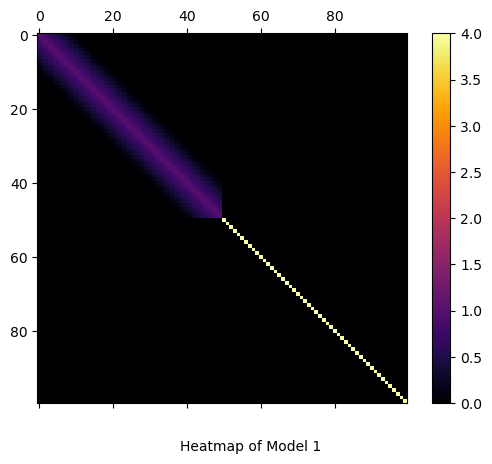
\includegraphics[scale=0.75]{simulation_result/pic_model1.png}
        \caption{Typical heatmap of Model 1 (banded matrix with ordering)}
        \label{fig:model1}
    \end{figure}
    \item Model 2 (sparse matrix without ordering). $\Sigma = \diag(A_1, A_2)$, where $A_2 = 4 I_{\frac{N}{2} \times \frac{N}{2}}$, $A_1 = B + \epsilon I_{\frac{N}{2} \times \frac{N}{2}}$, $B = [b_{ij}]_{\frac{N}{2} \times \frac{N}{2}}$, whose elements independently follow:
    \begin{equation}
        b_{ij} = \begin{cases}
            \text{Ber}(1, \frac{20}{N}) &\text{for}\hspace{2mm} i<j, \\
            1 & \text{for}\hspace{2mm}i=j, \\
            b_{ji} & \text{for}\hspace{2mm}i>j.
        \end{cases}
    \end{equation}
     Here $\text{Ber}(1, p)$ is a Bernoulli random variable that takes value 1 with probability $p$ and value 0 with probability $1-p$, and $\epsilon = \max(-\lambda_{\min} (B), 0) + 0.01$ to ensure that $A_1$ is positive definite. 
        \begin{figure}[H]
        \centering
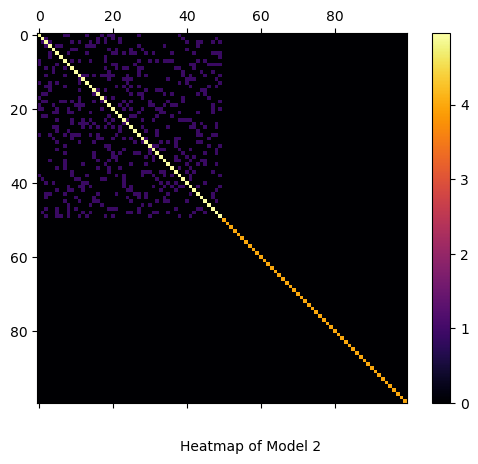
\includegraphics[scale=0.75]{simulation_result/pic_model2.png}
         \caption{Typical heatmap of Model 2 (sparse matrix without ordering)}
        \label{fig:model2}
    \end{figure}
\end{enumerate}

\subsection{Auxiliary Information}
In the simulation, we directly generate the estimates of the Location Indicator Matrix $L$ and the Relative Importance Indicator Matrix $C$, i.e., $\hat L$ and $\hat C$. The qualities of these estimates are tuned by some hyper-parameters. Table \ref{param-hatL} and \ref{param-hatC} list the descriptions of these hyper-parameters and the ranges of values they can take.
\begin{table}[htbp]
     \centering
     \begin{tabularx}{\textwidth}{c|X|c}
          \toprule
          Parameter & Description & Range \\ 
          \midrule
          \(l\) & Observation level, determines how we classify a pair \((i,j)\) as important, i.e., \(L_{ij} =1\). & 0.2 \\
          \(p\) & Conditional on \(L_{ij} =1\), the probability of actually observing \(\hat{L}_{ij} =1\). & 0.5, 0.8, 1 \\
          \(q\) & Conditional on \(L_{ij} = 0\), the probability of  observing \(\hat{L}_{ij} =1\). & 0, 0.1 \\
          \bottomrule
     \end{tabularx}
     \caption{hyper-parameters for Network Guided Thresholding Estimator}
     \label{param-hatL}
\end{table}
\vspace{10mm}
\begin{table}[htbp]
     \centering
     \begin{tabularx}{\textwidth}{c|X|c}
          \toprule
          Parameter & Description & Range \\ 
          \midrule
          $\eta$ & Accuracy rate of the order,  guarantees $S^{c_i}_{\lceil \eta k \rceil} \subseteq S^{\hat{c}_i}_{k}$ for all $1 \le k \le N$, where $c_i$ is the $i$-th column of $C$ and $\hat{c}_i$ is the $i$-th column of $\hat C$. Details of the algorithm to generate $\hat C$ can be found in \autoref{algo}.  & 0.1, 0.5, 0.8, 1 \\
          \bottomrule
     \end{tabularx}
     \caption{hyper-parameters for Network Guided Banding Estimator}
     \label{param-hatC}
\end{table}

\subsection{Numerical Results}
For each model described in \autoref{true_cov}, $T=100$ iid $N$-variate random vectors are generated from the normal distribution with mean 0 and covariance matrix $\Sigma$, for $N = 100, 300, 500$. For each setting of $(N, T, l, p, q)$ or $(N, T, \eta)$, 20 replications are used. We compare the numerical performance of the Network Guided Thresholding Estimator and the Network Guided Banding Estimator with a set of pure statistical methods including Sample Covariance Estimator, Soft Thresholding Estimator, Hard Thresholding Estimator, Linear Shrinkage Estimator, and Nonlinear Shrinkage Estimator. \autoref{res-model1} and \autoref{res-model2} list the numerical results under the Frobenius norm and the Matrix 2-norm. 

When the true covariance matrix is a banded one with order (model 1), both Network Guided estimators outperform other competitors as long as the auxiliary network information is decent. For the Network Guided Thresholding Estimator, it outperforms the sample covariance estimator, the hard thresholding estimator, and the linear shrinkage estimator for all $(p,q, N,T)$ combinations. However, to beat the soft thresholding estimator and the nonlinear shrinkage estimator, we will need $p,q$ to be not too large. In particular, type I error $q$ hurts the performance of the Network Guided Thresholding Estimator more than type II error $(1-p)$. When $q=0$, even if the probability of making the type II error is as large as $50\%$, it still performs better than other pure statistical methods. When it comes to the Network Guided Banding Estimator, it has smaller norms than all other pure statistical methods as long as the accuracy rate parameter $\eta$ is not too small. When $\eta=0.5$, the Network Guided Banding Estimator outperforms for most of the $(N,T)$ combinations. Given similar information quality, the Network Guided Banding Estimator performs better than the Network Guided Banding Estimator, which is consistent with the theory. We do not aim to compare the performances of the two Network Guided estimators as this is not a fair competition (the Network Guided Banding Estimator requires the auxiliary information to reveal the relative importance of neighbors for each node for this method to be applicable).

When the true covariance matrix is a sparse matrix without order (model 2), both Network Guided estimators again outperform other competitors when the auxiliary network information is decent. Now that our Network Guided Banding Estimator is applicable to a wider range of "bandable" matrix, it can be successfully applied under the setting of model 2. And it maintains its excellent performance given that the accuracy rate parameter $\eta$ is not too small. When $\eta=0.5$, the Network Guided Banding Estimator outperforms others for all the $(N,T)$ combinations. Even when $\eta=0.1$, its performance is still decent under this model setting. Similar to the previous setting, the Network Guided Thresholding Estimator as we are not making too much Type I error.  In summary, our simulation exercise shows the excellent numerical properties of the proposed Network Guided estimators. They both outperform other competitors as long as the auxiliary network information is decent. The performance of the Network Guided Thresholding Estimator is more sensitive to type I error than type II error. The Network Guided Banding Estimator, on the other hand, is not too sensitive to the accuracy rate parameter $\eta$, and it has excellent performance as long as $\eta$ is not too small.

\begin{landscape}
    % \resizebox{!}{0.45\textheight}{
        \begin{table}[H]
\centering
\caption{Simulation Results of Model 1}
\label{res-model1}
\resizebox{\linewidth}{0.2\textheight}{ %%%
% \resizebox{!}{0.9\textheight}{
\begin{tabular}{ll|p{2cm}p{2cm}p{2cm}p{2cm}p{2cm}p{2cm}p{2cm}p{2cm}p{2cm}p{2cm}p{2cm}p{2cm}p{2cm}p{2cm}p{2cm}}
\toprule
              &     & Network Guided Banding($\eta=1$) & Network Guided Banding ($\eta=0.8$) & Network Guided Banding ($\eta=0.5$) & Network Guided Banding ($\eta=0.1$) & Network Guided Thresholding ($(l, p, q)=(0.2, 1, 0)$) & Network Guided Thresholding ($(l, p, q)=(0.2, 1, 0.1)$) & Network Guided Thresholding ($(l, p, q)=(0.2, 0.8, 0)$) & Network Guided Thresholding ($(l, p, q)=(0.2, 0.8, 0.1)$) & Network Guided Thresholding ($(l, p, q)=(0.2, 0.5, 0)$) & Network Guided Thresholding ($(l, p, q)=(0.2, 0.5, 0.1)$) &       Sample & Soft Threshold & Hard Threshold & Linear Shrink & Nonlinear Shrink \\
Norm & $N$ &                                   &                                     &                                     &                                     &                                                       &                                                         &                                                         &                                                           &                                                         &                                                           &              &                &                &               &                  \\
\midrule
Frobenius Norm & 100 &                        5.73(0.30) &                          6.62(0.27) &                          8.84(0.39) &                         14.51(0.37) &                                            5.93(0.63) &                                              7.24(0.50) &                                              7.25(0.37) &                                                8.27(0.35) &                                              7.97(0.38) &                                                8.88(0.36) &  14.51(0.37) &     8.80(0.42) &    13.35(0.44) &   12.20(0.22) &       7.50(0.36) \\
              & 300 &                        7.96(0.22) &                         10.69(0.38) &                         15.41(0.38) &                         28.08(1.00) &                                           14.43(0.88) &                                             19.39(0.67) &                                             17.81(0.34) &                                               21.88(0.29) &                                             19.51(0.29) &                                               23.21(0.25) &  43.47(0.33) &    21.40(0.27) &    38.23(0.40) &   28.99(0.10) &             None \\
              & 500 &                        9.52(0.25) &                         13.45(0.27) &                         19.60(0.45) &                         36.45(1.04) &                                           22.26(0.65) &                                             31.18(0.53) &                                             27.56(0.47) &                                               34.96(0.41) &                                             30.10(0.43) &                                               36.87(0.39) &  72.42(0.42) &    32.82(0.41) &    62.41(0.55) &   41.31(0.10) &             None \\
Matrix-2 Norm & 100 &                        2.61(0.24) &                          2.64(0.35) &                          3.59(0.42) &                          4.48(0.52) &                                            1.77(0.25) &                                              2.02(0.24) &                                              2.09(0.27) &                                                2.31(0.25) &                                              2.39(0.39) &                                                2.54(0.37) &   4.48(0.52) &     3.18(0.45) &     3.90(0.44) &    3.75(0.37) &       3.55(0.43) \\
              & 300 &                        3.21(0.25) &                          3.82(0.34) &                          5.15(0.44) &                          7.73(0.57) &                                            2.74(0.25) &                                              3.42(0.21) &                                              3.36(0.16) &                                                3.96(0.15) &                                              3.63(0.16) &                                                4.19(0.16) &   9.24(0.34) &     3.94(0.23) &     7.37(0.21) &    5.60(0.21) &             None \\
              & 500 &                        3.21(0.28) &                          3.70(0.32) &                          5.36(0.41) &                          8.06(0.30) &                                            3.52(0.15) &                                              4.48(0.18) &                                              4.39(0.15) &                                                5.23(0.18) &                                              4.75(0.16) &                                                5.55(0.19) &  12.90(0.33) &     4.90(0.17) &    10.13(0.32) &    6.24(0.11) &             None \\
\bottomrule
\end{tabular}
}
\end{table}

        \begin{table}[H]
\centering
\caption{Simulation Results of Model 2}
\label{res-model2}
\resizebox{\linewidth}{0.2\textheight}{ %%%
\begin{tabular}{ll|p{2cm}p{2cm}p{2cm}p{2cm}p{2cm}p{2cm}p{2cm}p{2cm}p{2cm}p{2cm}p{2cm}p{2cm}p{2cm}p{2cm}p{2cm}}
\toprule
              &     & Network Guided Banding ($\eta=1$) & Network Guided Banding ($\eta=0.8$) & Network Guided Banding ($\eta=0.5$) & Network Guided Banding ($\eta=0.1$) & Networked Guided Thresholding ($(l, p, q)=(0.2, 1, 0)$) & Networked Guided Thresholding ($(l, p, q)=(0.2, 1, 0.1)$) & Networked Guided Thresholding ($(l, p, q)=(0.2, 0.8, 0)$) & Networked Guided Thresholding ($(l, p, q)=(0.2, 0.8, 0.1)$) & Networked Guided Thresholding ($(l, p, q)=(0.2, 0.5, 0)$) & Networked Guided Thresholding ($(l, p, q)=(0.2, 0.5, 0.1)$) &        Sample & Soft Threshold & Hard Threshold & Linear Shrink & Nonlinear Shrink \\
Norm & $N$ &                                   &                                     &                                     &                                     &                                                         &                                                           &                                                           &                                                             &                                                           &                                                             &               &                &                &               &                  \\
\midrule
Frobenius Norm & 100 &                        9.95(0.26) &                         10.88(0.27) &                         14.69(0.22) &                         19.57(0.40) &                                             10.35(1.65) &                                               12.83(1.29) &                                               16.22(0.60) &                                                 17.56(0.59) &                                               17.84(0.57) &                                                 18.95(0.56) &   25.94(0.49) &    19.03(0.52) &    25.71(0.51) &   16.26(0.27) &      15.20(0.32) \\
              & 300 &                       16.91(0.31) &                         18.52(0.35) &                         24.30(0.28) &                         33.88(0.27) &                                             26.82(4.30) &                                               36.72(2.80) &                                               45.48(0.92) &                                                 50.98(0.83) &                                               50.26(0.87) &                                                 54.94(0.82) &   83.47(0.63) &    53.95(0.70) &    81.89(0.68) &   33.76(0.10) &             None \\
              & 500 &                       20.39(0.30) &                         22.10(0.29) &                         30.03(0.19) &                         43.37(0.09) &                                             36.56(6.83) &                                               55.55(4.45) &                                               69.88(1.26) &                                                 79.87(1.04) &                                               76.96(0.85) &                                                 85.64(0.80) &  137.19(0.60) &    82.93(0.71) &   133.60(0.66) &   44.59(0.07) &             None \\
Matrix-2 Norm & 100 &                        3.52(0.28) &                          3.61(0.35) &                          5.13(0.35) &                          8.65(0.50) &                                              3.01(0.61) &                                                3.42(0.59) &                                                4.43(0.45) &                                                  4.73(0.46) &                                                4.81(0.43) &                                                  5.06(0.44) &    7.05(0.59) &     5.00(0.41) &     6.98(0.59) &    6.82(0.66) &       5.67(0.89) \\
              & 300 &                        3.66(0.15) &                          3.66(0.17) &                          5.09(0.22) &                          9.05(0.25) &                                              5.00(0.80) &                                                6.12(0.67) &                                                8.35(0.47) &                                                  9.17(0.47) &                                                9.18(0.51) &                                                  9.91(0.51) &   15.48(0.66) &     9.58(0.51) &    15.06(0.63) &    9.08(0.23) &             None \\
              & 500 &                        3.97(0.17) &                          4.04(0.14) &                          4.58(0.16) &                          8.78(0.07) &                                              5.26(1.04) &                                                7.00(0.93) &                                               10.52(0.27) &                                                 11.76(0.26) &                                               11.59(0.21) &                                                 12.72(0.21) &   21.43(0.38) &    12.25(0.25) &    20.58(0.36) &    9.41(0.13) &             None \\
\bottomrule
\end{tabular}
}
\end{table}

    % }
\end{landscape}


\section{Empirical Application (preliminary)}
We apply the two Network Guided Estimators to factor model residual covariance matrix. Assume that the excess returns have the following factor structure
\begin{equation*}
    Y_{it} = B_{i}'F_{t} + \epsilon_{it}
\end{equation*}
and we assume that \(\Sigma = [E \epsilon_{i} \epsilon_{j}]_{1 \leq i,j\leq N}\) is sparse.

We collect daily return data on SP500 stock from 2004 to 2015 from CRSP, together with daily data on Fama-French 3 factors and the risk free rate.  We do a rolling window analysis, each window consists of an estimation period of 252 days and a testing period of 21 days. In the estimation period, we estimate the factor loadings by linear time series regression of excess return \(Y_{it}\) on \(F_{t}\), hence allowing the betas to vary over time, and find the de-factored excess return by 
\begin{equation*}
    \hat{\epsilon}_{it} = Y_{it} - \hat{B}_{i}'F_{t},
\end{equation*}
and we estimate \(\Sigma_{\epsilon}\) by the Network Guided Estimator applied to \(\hat{\Sigma}_{\epsilon} = \frac{1}{T} \sum_{t}\hat{\epsilon}_{t} \hat{\epsilon}_{t}'\).


We now introduce the auxiliary network information that we use. The first network we have is the \textit{News-Implied Network}. The news data are obtained from RavenPack Equity files Dow Jones Edition for the period January 2004 to December 2015. This comprehensive news dataset combines relevant content from multiple sources, including Dow Jones Newswires, Wall Street Journal, and Barron's MarketWatch, which produce the most actively monitored streams of news articles in the financial system. Each unique news story (identified by a unique story ID) tags the companies mentioned in the news by their unique and permanent entity identifier codes (RP\_ENTITY\_ID),  by which we link to stock identifier TICKER and PERMNO. Same as \cite{ge2022news}, we identify links by news co-mentioning. That is, if a piece of business news reports two companies together, they share a link. We do not consider the news that co-mention more than two companies since although they may carry potential information about links, they provide noisier information. We also remove news with topics including analyst recommendations, rating changes, and index movements, as these types of news might stack multiple companies together when they actually do not have real links. \autoref{table:news} and \autoref{table:freq} in Apprendix provide descriptive statistics for RavenPack Equity files Dow Jones Edition dataset during the sample period. Since our comprehensive news dataset combines several sources, given a similar length of sample period, the number of unique news stories is more than ten times larger than that from \cite{scherbina2015economic} and more than eight hundred times than that from \cite{schwenkler2019network}. For link identification purposes, we only use sample news (1) are not about topics mentioned above, (2) tag $S\& P$ $500$ companies and (3) mention exactly two companies, which is a subsample of $1,637,256$ unique news stories. The second network we consider is the \textit{Analyst Coverage Network}.  It has been documented that shared analyst coverage is a strong proxy for fundamental linkages between firms and reflects firm similarities along many dimensions (\cite{ali2020shared}, \citet{israelsen2016does}, \citet{kaustia2013common}). We use the Institutional Brokers Estimate System (IBES) detail history files to construct the analyst co-coverage-based adjacency matrix. For each year in the sample, we consider a stock is covered by an analyst if the analyst issues at least one FY1 or FY2 earnings forecast for the stock during the year. And we consider two stocks as linked if there are common analysts during the year, weighted by the number of common analysts. We then add up the yearly adjacency matrices to get the full sample adjacency matrix.  We also consider a couple of \textit{Industry-Based Networks}. This is motivated by \cite{moskowitz1999industries}, \citet{engelberg2018know} that stocks within the same industry exhibit excess co-movement.  Utilizing this fact in the estimation of large covariance matrices, \cite{fan2016incorporating} apply location-based thresholding based on GICS sector classification. We consider industry classification based on The Standard Industrial Classification (SIC). In particular, we consider two stocks to be linked if they have the same 4-digit (3-digit) SICCD code, and thus we have two block-diagonal network matrices where companies within the same industry are fully connected. Lastly, we consider a \textit{Customer-Supplier Network} (\cite{cohen2008economic}). The links are obtained from Andrea Frazzini's data library, where strength of links is weighted by sales.

To demonstrate the usefulness of auxiliary network information in capturing pairs with non-zero correlations, we plot the histograms of factor model residual correlations for all non-diagonal elements (all possible pairs among entities) and only the linked pairs (implied by the aforementioned auxiliary network information). \autoref{fig:corr5factors} show the histograms of Fama-French 5-factor model residual correlations. From the top left plot, we find that after removing five FF factors, the remaining correlations are mostly zero or take small values around zero. In contrast, the correlation distributions are positively skewed among linked pairs, 
and the probability of having zero correlation is much lower. Taking the upper right plot as an example, most of the stock pairs that are co-covered by analysts have positive residual correlations, and the number of pairs having zero correlation is very small (i.e., type I error is small). This indicates that our auxiliary network information is useful in identifying the pairs with non-zero correlations. In \autoref{fig:corr5factors} of the Appendix, we plot the histograms of residual correlations after removing five principal components, and similar patterns are found.
\begin{figure}[H]
    \centering
    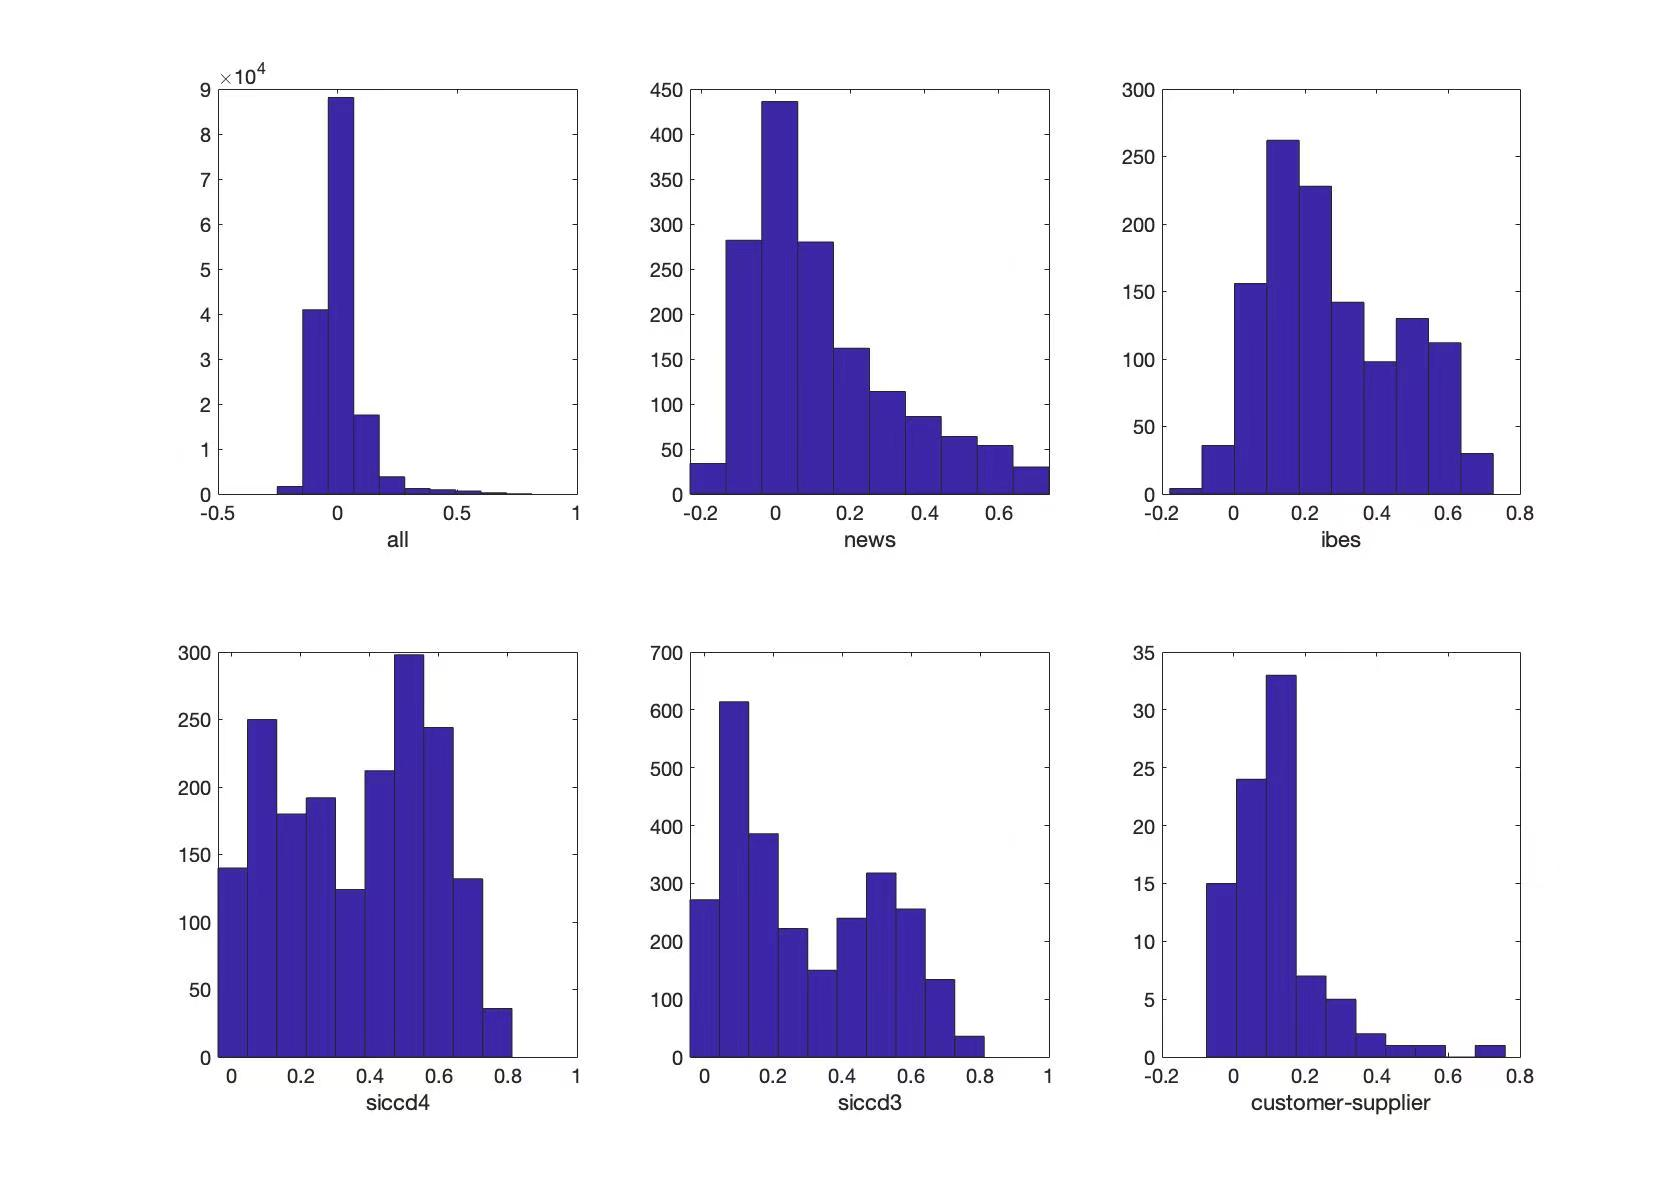
\includegraphics[scale=0.25]{pic/corr_5factors.jpg}
    \caption{Histograms of factor model residual correlations. Correlations are calculated on the Fama-French 5-factor model residuals. The top left sub-figure shows the histogram of all non-diagonal residual correlations. The rest sub-figures show the histograms of residual correlations among linked pairs.}
    \label{fig:corr5factors}
\end{figure}

Next, we apply the proposed method to a portfolio management problem. In particular, we consider the estimation of Global Minimum Variance (GVM) portfolio as in \cite{ledoit2004HoneyShrunk}. The key is to estimate the covariance matrix of asset returns (i.e.,$\Sigma_{Y}$) as weight of such portfolio is given by
\begin{equation*}
    w = \frac{\Sigma_{Y} \mathbf{1}}{\mathbf{1}' \Sigma_{Y} \mathbf{1}},
\end{equation*}
where \(\mathbf{1}\) is a conforming vector of ones. Given the factor structure,  we have
\begin{equation*}
    \Sigma_{Y} = B \Sigma_{F} B' + \Sigma_{\epsilon}
\end{equation*}
We do a rolling window analysis, where each window consists of an estimation period of 252 days and a testing period of 21 days. In the estimation period, we first estimate the factor model, and then apply Network Guided Estimator to the factor model residual covariance matrix. Having \(\hat{B} ,\hat{\Sigma}_{F}, \hat{\Sigma}_{\epsilon}\), we then construct $\hat{\Sigma}_{Y} = \hat{B} \hat{\Sigma}_{F} \hat{B}' + \hat{\Sigma}_{\epsilon}$ and derive the \textit{global minimum variance} portfolio where weights are $w = \frac{\hat{\Sigma}_{Y} \mathbf{1}}{\mathbf{1}' \hat{\Sigma}_{Y} \mathbf{1}}$.  We collect the portfolio return over the next 21-day testing period. This constitutes one of the rolling windows. Then we move forward 21 days and repeat this exercise. Using 2004- 2014 daily data, we can construct a daily portfolio return from 2005 to 2015, where the portfolio is re-balanced every 21 days. We compute the holding period return of this portfolio and its standard deviation. The results are summarized in \autoref{table:GVP}. 
\begin{table}[H]
    \centering
    \begin{tabular}{lr}
\toprule
Estimator &  Out-of-sample standard deviation of GMV portfolio              \\
\midrule
Network Guided Thresholding      &              0.0255  \\
Linear Shrinkage       &               0.0264\\
Universal Thresholding &                0.0263  \\
Equally Weighted        &        0.0667\\
\bottomrule
\end{tabular}
    \caption{Out-of-sample performance of each method}
    \label{table:GVP}
\end{table}
As discussed in \cite{engle2019large} and \cite{chen2019new}, 
to judge the performance of a covariance matrix estimation method by the global minimum variance (GMV) portfolio, the most important measure is the constructed portfolio's out-of-sample volatility. In this respect, the global minimum variance portfolio constructed using the covariance matrix estimated using \textit{Network Guided Thresholding} has the smallest out-of-sample standard deviation.  Notice that the empirical results are preliminary, and we are still figuring out how to utilize those auxiliary better information. 

\section{Conclusion}
In the era of big data, we are gaining access to more and more auxiliary information apart from the observations of $\{\boldsymbol{X}_t\}_{t=1}^T$, which could potentially help us learn about the underlying structure of the covariance matrix (i.e., connectivity among entities). We believe this is the first paper that incorporates complex network information into the estimation of large covariance matrices. We believe a similar idea can be extended to many other settings, like the estimation of large dynamic covariance matrices. For example, dynamic network information could be well incorporated into the conditioning information set in \cite{chen2019new}.
\bibliographystyle{abbrvnat.bst}
\bibliography{ref}

\begin{appendices}
% \section{Appendix}
\section{Supplementary figures and tables}
\begin{table}[H]
\centering\renewcommand\cellalign{lc}
\setcellgapes{3pt}\makegapedcells
\begin{tabular}{|l|l|} \hline
  \makecell{Number of unique news stories} &$88,316,898$\\ 
  \makecell{Number of stories remaining after removing topics including\\ analyst recommendations, ratings changes, and index movements}&$87,841,641$\\
  \hspace{3mm}Of these: &\\
  \hspace{3mm}Number of stories tag sample companies& $8,341,848 $\\
  \hspace{5mm}Of these: &\\
  \hspace{5mm}Number of stories that mention only one company& $5,507,772 \hspace{1mm}(66.03\%)$\\
  \hspace{5mm}Number of stories that mention exactly two companies& $1,637,256 \hspace{1mm}(19.63\%) $ \\
  \hspace{5mm}Number of stories that mention more than two companies&$1,196,820 \hspace{1mm}(14.34\%)$ \\
\hline\end{tabular}
\caption{Descriptive statistics for RavenPack Equity files Dow Jones Edition for the period January 2004 to December 2015.}
\label{table:news}
\end{table}


\begin{table}[H]
    \centering
  \begin{tabular}{cccc}
  \hline
  Number of yearly window a pair gets identified& Frequency & Percentage& Cumulative Percentage\\
0   & 217024&      $72.80\%$ & $72.80\%$\\ 
1 &          40178   &   $13.48\%$ & $86.28\%$ \\ 
2     &      13302 &     $4.46\%$ & $90.74\%$\\ 
3         &  7116    &  $2.39\%$ & $93.13\%$\\ 
4      &     4522   &   $1.52\%$ & $94.65\%$\\ 
5        &   3236     & $1.09\%$ & $95.74\%$\\ 
6       &    2506    &$0.84\%$ & $96.58\%$\\ 
7        &   2022    & $0.68\%$ & $97.26\%$\\ 
8         &  1804   &  $0.61\%$ & $97.87\%$\\ 
9          & 1508   &  $0.51\%$ & $98.38\%$\\ 
10          & 1350    & $0.45\%$ & $98.83\%$\\ 
11           &1232     &$0.41\%$ & $99.24\%$\\ 
12           &2316     & $0.78\%$& $100\%$\\ 
\hline
\end{tabular}
\caption{Frequency distribution table of the number of yearly link identification windows that a pair gets identified as economic neighbors for all possible pairs $(i,j)$ in our sample. Note: A pair identified in $k$ yearly windows could get multiple co-mentions within each window. }
\label{table:freq}
\end{table}


\begin{figure}[H]
    \centering
    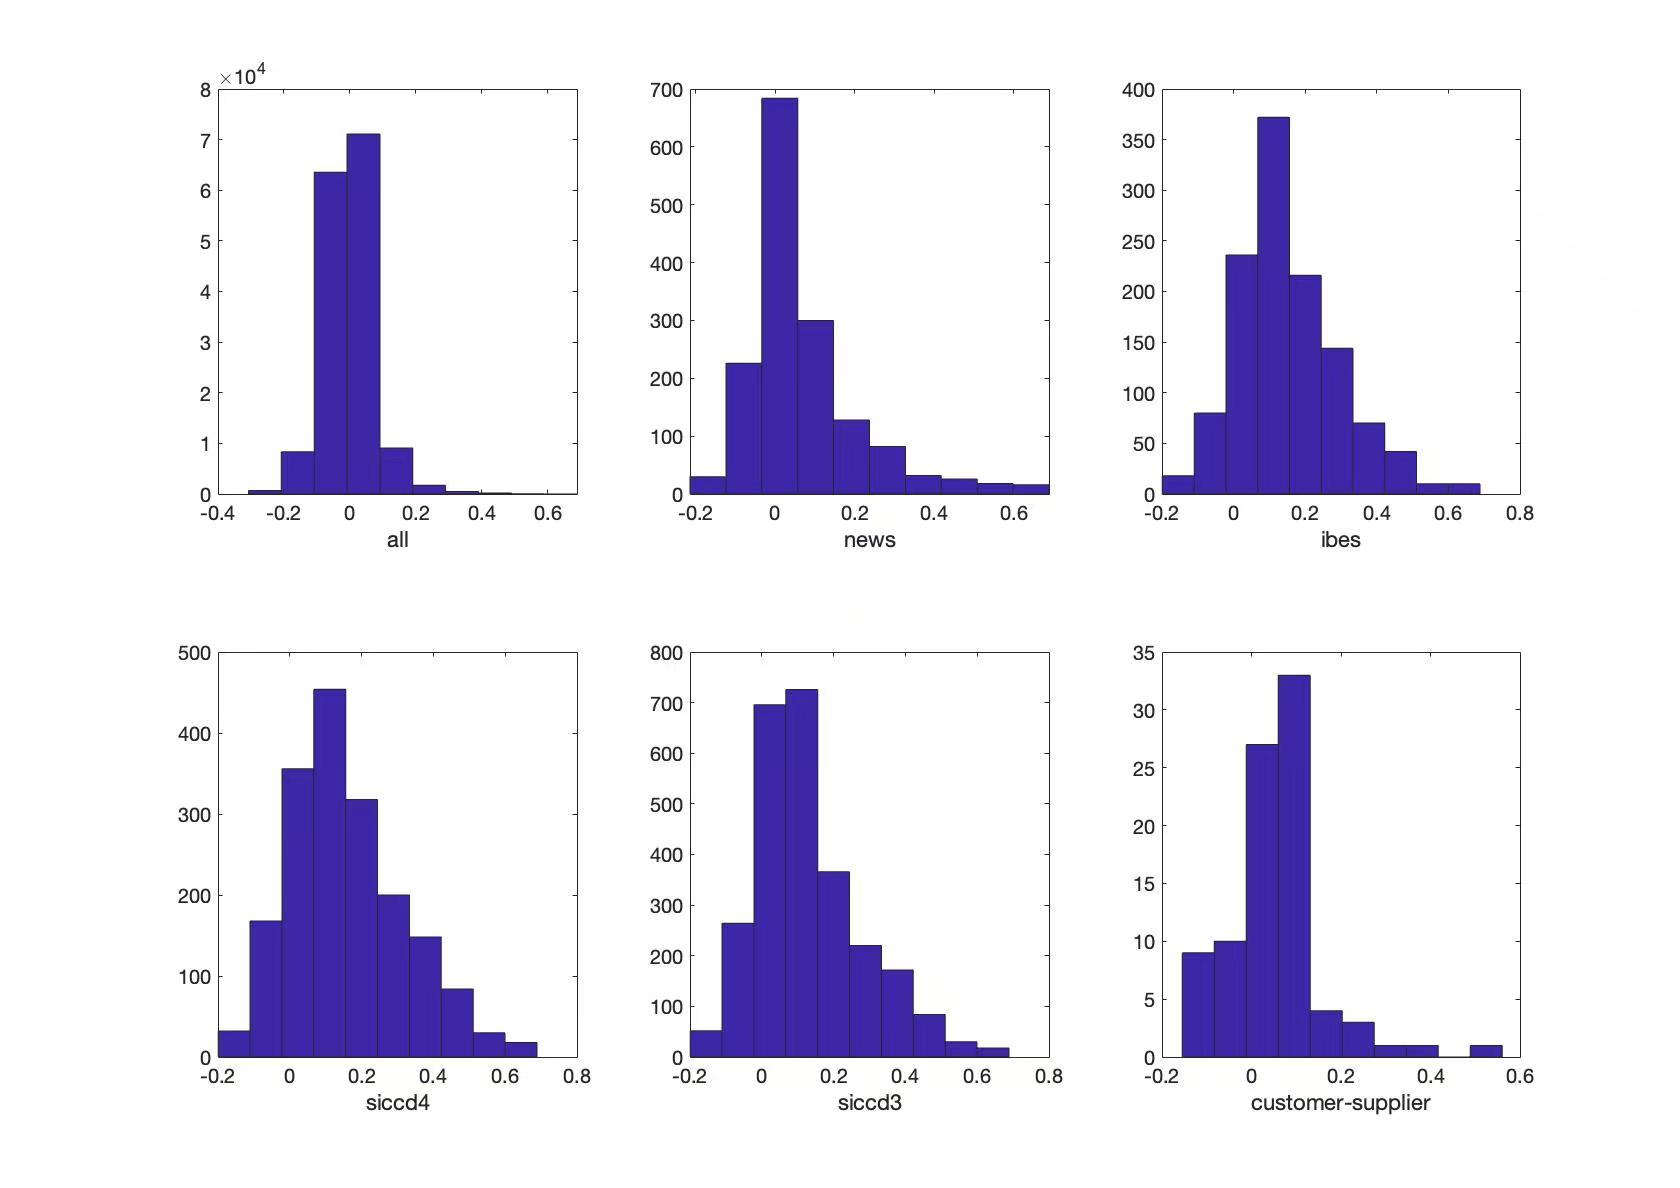
\includegraphics[scale=0.25]{pic/corr_5pca.jpg}
    \caption{Histograms of factor model residual correlations. Correlations are calculated on the residuals after removing five principal components. The top left sub-figure shows the histogram of all non-diagonal residual correlations. The rest sub-figures show the histograms of residual correlations among linked pairs.}
    \label{fig:corr5_pca}
\end{figure}


\section{Proof of Theorem 1}
\begin{proof}{ of Theorem \ref{theorem1}}

    Suppose \(F\) is Gaussian and for sufficiently large \(M\), 
    \begin{equation*}
            \lambda = M \sqrt{\frac{\log N}{T}}
    \end{equation*}
    and \(\frac{\log N}{T} \to 0\) as \(T \to \infty\), 
    then for the operator norm \(\norm{M}= \max_{j} \abs{\lambda_{j}(M)}\) where \(\lambda_{1},\dots,\lambda_{N}\) are the eigenvalues of \(M\), \autoref{theorem1} establishes that
        \begin{equation*}
      \norm{T_{\hat{L},\lambda}\pqty{\hat{\Sigma}} - \Sigma } = O_{p}\pqty{c_{1}(p) \sqrt{\frac{\log N}{T}}+c_{0}(p)\pqty{\frac{\log N}{T}}^{\frac{1-q}{2}}}
       \end{equation*}
    Consider the following decomposition:
    \begin{equation*}
        \norm{T_{\hat{L},\lambda}\pqty{\hat{\Sigma}} - \Sigma } \leq \norm{T_{\hat{L} ,\lambda}(\Sigma) - \Sigma} +\norm{T_{\hat{L}, \lambda}(\hat{\Sigma}) - T_{\hat{L},\lambda}(\Sigma)} = \mathbf{I} + \mathbf{II}
    \end{equation*}
    The first term can be bounded by 
    \begin{align*}
        \mathbf{I} &\leq \max_{i} \sum_{j} \abs{s_{\hat{L}, \lambda}(\sigma_{ij}) - \sigma_{ij}} \\
        &= \max_{i} \sum_{j} \hat{L}_{ij}^{0} \abs{s_{\lambda}(\sigma_{ij}) - \sigma_{ij}}\\
        &= \max_{i} \sum_{j} \bqty{L_{ij}^{0} \abs{s_{\lambda}(\sigma_{ij}) - \sigma_{ij}} + (\hat{L}_{ij}^{0} - L_{ij}^{0})\abs{s_{\lambda}(\sigma_{ij}) - \sigma_{ij}}} \\
        &\leq (1 + o_{p}(1))\max_{i} \sum_{j} \bqty{L_{ij}^{0} \abs{s_{\lambda}(\sigma_{ij}) - \sigma_{ij}}}\\
        &\leq (1 + o_{p}(1))\max_{i} \sum_{j} \bqty{L_{ij}^{0} \abs{\sigma_{ij} \mathbf{1}\Bqty{\sigma_{ij}\leq \lambda} + (s_{\lambda}(\sigma_{ij}) - \sigma_{ij}) \mathbf{1}\Bqty{\sigma_{ij} > \lambda}}}\\
        &\leq (1 + o_{p}(1)) \max_{i} \sum_{j} \bqty{L_{ij}^{0}\abs{\sigma_{ij}}^{q} \lambda^{1 -q}}\\
        &\leq (1 + o_{p}(1)) c_{0}(p) \lambda^{1-q}
    \end{align*}
    And the second term can be bounded similar to \cite{rothman2009generalized}, 
    \begin{align*}
        \mathbf{II} &\leq  \max_{i} \sum_{j} \bqty{\hat{L}_{ij}^{1} \abs{\hat{\sigma}_{ij} - \sigma_{ij}} + \hat{L}_{ij}^{0} \abs{s_{\lambda}(\hat{\sigma}_{ij}) - s_{\lambda} (\sigma)_{ij}}}\\
        &\leq (1 + o_{p}(1))c_{1}(p)\max_{ij} \abs{\hat{\sigma}_{ij} - \sigma_{ij}} + (1 + o_{p}(1)) \max_{i} \sum_{j} L_{ij}^{0} \abs{s_{\lambda}(\hat{\sigma}_{ij}) - s_{\lambda} (\sigma)_{ij}} \\
        &= O_{p}\pqty{c_{1}(p) \sqrt{\frac{\log N}{T}} + c_{0}(p) \pqty{\lambda^{1-q} + \lambda^{-q} \sqrt{\frac{\log N}{T}}}} \\
    \end{align*}
    Hence we have 
    \begin{align*}
        \norm{T_{\hat{L},\lambda}\pqty{\hat{\Sigma}} - \Sigma } &= O_{p}\pqty{c_{1}(p) \sqrt{\frac{\log N}{T}} + c_{0}(p) \pqty{\lambda^{1-q} + \lambda^{-q} \sqrt{\frac{\log N}{T}}}} \\
        &= O_{p}\pqty{c_{1}(p) \sqrt{\frac{\log N}{T}} + c_{0}(p)\pqty{\frac{\log N}{T}}^{\frac{1-q}{2}}}
    \end{align*}
\end{proof}


\section{Proof of Theorem 2 and 3}
\begin{lemma}
    For a series $\{ a_n \geq 0 \}$, denote $a_{(i)}$ as the $i$-th largest element. If $\sum_{i=k+1}^\infty a_{(i)} = O(k^{-\alpha})$, then $a_{(k)} = O(k^{-\alpha-1})$.
    \label{lemma_sum_single}
\end{lemma}

\begin{lemma}
    If $X_n = O_P(Y_n)$ and $Y_n = O_P(a_n)$, then $X_n = O_P(a_n)$. If $X_n = O_P(a_n)$ and $Y_n = O_P(b_n)$, then $X_n Y_n = O_P(a_n b_n)$.
    \label{lemma_OP}
\end{lemma}

\begin{proof}{ of Lemma \ref{lemma_OP}}

    (1)
    $\forall \epsilon, \exists M_1(\epsilon), N_1(\epsilon), \forall n > N_1, \Pr \{ |X_n/Y_n| > M_1 \} < \epsilon $. Similarly, $M_2(\epsilon)$ and $N_2(\epsilon)$ for $Y_n = O_P(a_n)$. If we choose $M = \max\{ M_1^2(\frac{\epsilon}{2}), M_2^2(\frac{\epsilon}{2}) \}$ and $N = \max \{ N_1(\frac{\epsilon}{2}), N_2(\frac{\epsilon}{2}) \}$, then $\forall n > N(\epsilon)$ we have 
    \begin{equation}
        \begin{split}
            \Pr \{ |\frac{X_n}{a_n}| > M \} &= \Pr\{ |\frac{X_n}{Y_n}| > \sqrt{M} \ \land \ |\frac{X_n}{a_n}| > M \} + \Pr \{ |\frac{X_n}{Y_n}| \leq \sqrt{M} \ \land \ |\frac{X_n}{a_n}| > M \} \\
            &\leq \Pr \{ |\frac{X_n}{Y_n}| > \sqrt{M} \} + \Pr \{ |\frac{Y_n}{a_n}| > \sqrt{M} \} \\
            &< \epsilon
        \end{split}
    \end{equation}

    (2)
    $\forall \epsilon, \exists M_1(\epsilon), N_1(\epsilon), \forall n>N_1, \Pr \{ |X_n/a_n| > M_1 \} < \epsilon $. Similarly, $M_2(\epsilon)$ and $N_2(\epsilon)$ for $Y_n = O_P(b_n)$. If we choose $M = \max\{ M_1^2(\frac{\epsilon}{2}), M_2^2(\frac{\epsilon}{2}) \}$ and $N = \max \{ N_1(\frac{\epsilon}{2}), N_2(\frac{\epsilon}{2}) \}$, then $\forall n>N(\epsilon)$ we have
    \begin{equation}
        \begin{split}
            \Pr \{ |\frac{X_n Y_n}{a_n b_n}| > M \} &=  
                \Pr \{ |\frac{X_n}{a_n}| > \sqrt M \ \land\ |\frac{X_n Y_n}{a_n b_n}| > M  \} + 
                \Pr \{ |\frac{X_n}{a_n}| \leq \sqrt M \ \land\ |\frac{X_n Y_n}{a_n b_n}| > M  \} \\
            &\leq  \Pr \{ |\frac{X_n}{a_n}| > \sqrt M \} + 
                \Pr \{ |\frac{Y_n}{b_n}| > \sqrt M \} \\
            &< \epsilon.
        \end{split}
    \end{equation}
\end{proof}

%\proof{ of theorem \ref{theorem2}}
\begin{proof}{ of Theorem \ref{theorem2}}

    Denote $B_{R, k}(\hat R) = B_{C, k}(\hat R) = [\hat r_{ij} I(j\in S_{k}^{c_i} \land i\in S_{k}^{c_j})]$, and substituting $\hat r_{ij}$ with $r_{ij}$ yields $B_{C, k}(R)$. The notations are consistent with (\ref{network banding estimator}). We decompose as follows: 
    \begin{equation}
    	\begin{split}
            \lVert B_{\hat{C}, k}(\hat R) - R \rVert &\leq 
                \lVert B_{\hat{C}, k}(\hat R) - B_{\hat{C}, k}(R) \rVert + 
            	\lVert  B_{\hat{C}, k}(R) - B_{C, k}(R) \rVert + 
                \lVert B_{C, k}(R) - R \rVert \\
            &= \mathrm{I} + \mathrm{II} + \mathrm{III},
        \end{split} 
        \label{decompose}
    \end{equation}
        
    Bound term $\mathrm{I}$. 
    \begin{equation}
    	\begin{split}
    	    \mathrm{I} &\leq \| B_{\hat{C}, k}(\hat R) - B_{\hat{C}, k}(R) \|_{(\infty, 
    	        \infty)} \\
        	&= \max_i \Sigma_{j:\ j\in S_{k}^{\hat c_i} \land i\in S_{k}^{\hat c_j}} |\hat 
        	    r_{ij} - r_{ij}| \\
            &\leq (\max |S_{k}^{\hat c_i}|)  (\max_{i,j} 
                |\hat r_{ij} - r_{ij}|)  \\
            &= O_P(k \sqrt\frac{\log N}{T}). 
    	\end{split}  
    	\label{I res}
      \end{equation}
    Bound term $\mathrm{III}$. 
    \begin{equation}
        \begin{split}
    	    \mathrm{III} &\leq \max_i \Sigma_{j:\ j \notin S_{k}^{c_i} \lor i 
    	        \notin  S_{k}^{c_j}} |r_{ij}| \\
        	&\leq \max_i \Sigma_{j:\ j \notin S_{k}^{c_i}} |r_{ij}| + \max_i \Sigma_{j:\
        	    j\in S_{k}^{c_i} \land i\notin S_{k}^{c_j}} |r_{ij}|  \\
    		&= \mathrm{III_1} + \mathrm{III_2}.
        \end{split}  
        \label{III}  
    \end{equation}
    By lemma \ref{lemma_sum_single}, we have 
    \begin{equation}
    	\begin{split}
    		\mathrm{III_1}  &= O(  c_0(N) \Sigma_{i=k}^p 
    		    i^{-\alpha-1}  ) \\
      	    &= O( c_0(N) k^{-\alpha} )
        \end{split}
    \end{equation}
    and 
    \begin{equation}
    	\begin{split}
    		\mathrm{III_2} &\leq |S_{k}^{c_i}| ( \max_{i,j:\ i\notin S_{k}^{c_j}} |r_{ij}| )     \\
            &= k \ O( c_0(N) k^{-\alpha-1})  \\
            &= O( c_0(N) k^{-\alpha} ).
    	\end{split}
    \end{equation}
    So we conclude 
    \begin{equation}
        \mathrm{III} = O( c_0(N) k^{-\alpha} ). 
        \label{III res}
    \end{equation}
        
    Bound term $\mathrm{II}$. We denote 
    \begin{equation}
    	\begin{split}
    		A_{k} &:= \{ (i,j) | j\in S_{k}^{c_i} \land i \in S_{k}^{c_j} \} \\
            \hat A_k &:= \{ (i,j) | j\in S_{k}^{\hat c_i} \land i \in S_{k}^{\hat c_j} \}, 
    	\end{split}
    \end{equation}
    We further decompose $\mathrm{II}$ as: 
    \begin{equation}
    	\begin{split}
    		\mathrm{II} &\leq \max_i \Sigma_{j:\ (i,j)\in A_k \triangle \hat A_k }       |r_{ij}| \\
            &\leq \max_i \Sigma_{j:\ (i,j) \in (A_k - \hat A_k)} |r_{ij}| + 
            	\max_i \Sigma_{j:\ (i,j) \in (\hat A_k - A_k)} |r_{ij}| \\
            &= \mathrm{IV} + \mathrm{V}.
    	\end{split}
        \label{II decompose}
    \end{equation}    
    Because $(\hat A_k - A_k) \subseteq \overline{A_k}$, term $\mathrm{V} = O_P(c_0(N) k^{-\alpha})$ can be bounded in the same way as $\mathrm{III}$. To bound term $\mathrm{IV}$, notice that the equation in assumption \ref{asmp:framework2} indicates 
    \begin{equation}
    	\begin{split}
    	    & \forall i, S_{\lceil \eta k \rceil}^{c_i} \subseteq S_{k}^{\hat c_i} \\
            \Rightarrow & \\
            & A_k - \hat A_k \subseteq \overline{ A_{\lceil \eta k \rceil} }  \\
            \Rightarrow & \\
    		& \mathrm{IV} \leq \max_i \Sigma_{j:\ (i,j)\in\overline{A_{\lceil \eta k \rceil}}} |r_{ij}| := \mathrm{III'}  \\
            %\Rightarrow & \\
            % & \mathrm{IV} = O( \mathrm{III} ).
    	\end{split}
     \label{impli:asmp:framework2}
    \end{equation} 
    By (\ref{impli:asmp:framework2}) and (\ref{asmp:framework2}), we have $\mathrm{IV} = O_P (\mathrm{III'})$. Similarly as $\mathrm{III}$, it is easy to show $\mathrm{III'} = O( c_0(N) k^{-\alpha} ) $. Then together with \autoref{lemma_OP}, we have
    \begin{equation}
        \begin{split}
            \mathrm{IV} &= O_P( \mathrm{III} ) \\
            &= O_P(c_0(N) k^{-\alpha}) .
        \end{split} 
        \label{VI}
    \end{equation}
    To sum up, 
    \begin{equation}
    	\mathrm{II} = O_P( c_0(N) k^{-\alpha}  ). 
    	\label{II res}
    \end{equation}
    By (\ref{I res}), (\ref{II res}), (\ref{III res}) and (\ref{k_NT}), we attain the rate in (\ref{theorem2_R_rate}).
    
    Now consider the covariance estimation error. Similar to the argument in (\cite{liu2014EC2})'s Appendix E, we have 
    \begin{equation}
    	\begin{split}
    		B_{\hat C, k}(\hat \Sigma) - \Sigma =& \hat D B_{\hat C, k}(\hat R) \hat D - DRD \\
            =& (\hat D - D) R D + (\hat D - D) (B_{\hat C, k}(\hat R) - R) D + (\hat D - D) (B_{\hat C, k}(\hat R) - R) (\hat D - D) + \\
        	& (\hat D - D) R (\hat D - D) + D (B_{\hat C, k}(\hat R) - R) D + D (B_{\hat C, k}(\hat R) - R) (\hat D - D) + \\
            & DR(\hat D - D)
    	\end{split}
        \label{cov decompose}
    \end{equation}
    Then by $\|AB\|_2 \leq \|A\|_2 \|B\|_2$ we have 
    \begin{equation}
        \begin{split}
            \lVert B_{\hat C, k}(\hat \Sigma) - \Sigma \rVert_2 \leq & 
                \underbrace{ 2 \lVert \hat D -	D \rVert_2 \lVert R \rVert_2 \lVert D \rVert_2 }_{T_1} + 
                \underbrace{ 2\lVert \hat D - D \rVert_2 \lVert B_{\hat C, k}(\hat R) - R \rVert_2 \lVert D \rVert_2 }_{T_2} \\
            & + \underbrace{ \lVert \hat D - D \rVert_2^2 \lVert B_{\hat C, k}(\hat R) - R \rVert_2 }_{T_3} + 
                \underbrace{ \lVert \hat D - D \rVert_2^2 \lVert R \rVert_2 }_{T_4} + 
                \underbrace{ \lVert B_{\hat C, k}(\hat R) - R \rVert_2 \lVert D \rVert_2^2 }_{T_5} \\
            \leq & \underbrace{ 2 \sqrt{\kappa} \lambda_{\max } (R) \eta_1     }_{T_1} + 
                \underbrace{ 2\sqrt{\kappa} \eta_1 \eta_2}_{T_2} + 
                \underbrace{ \eta_1^2 \eta_2 }_{T_3} + 
                \underbrace{ \lambda_{\max}(R) \eta_1^2 }_{T_4} + 
                \underbrace{\kappa \eta_2}_{T_5} .
        \end{split}
        \label{cor2cov 2}
    \end{equation}
    where $\eta_1 =  \lVert \hat D - D \rVert_2 = O_P( \sqrt\frac{\log N}{T} )$ is given by assumption \ref{Gaussian asmp}, $\eta_2 = \lVert B_{\hat C, k}(\hat R) - R \rVert_2$ is already known, and $\lambda_{\max} (R) \leq 1/\varepsilon$. Because we assume $\eta_1$ and $\eta_2$ tend to $0$, we have  
    \begin{equation}
        \begin{split}
            \lVert \hat B_{\hat C, k}(\hat \Sigma) - \Sigma \rVert_2 
                = O( T_5 ) 
            = O_P (  
                c_0(N)^\frac{1}{\alpha+1}  
                ( \frac{\log N}{T} )^\frac{\alpha}{2(\alpha+1)}  ) \\
        \end{split}	
    \end{equation}
\end{proof}

\begin{proof}{ of Theorem \ref{theorem3}}

    We can decompose in the same way as (\ref{decompose}). 
    \begin{equation}
    	\begin{split}
            \lVert B_{\hat{C}, k}(\hat R) - R \rVert_F^2 &\leq 
                3 (\lVert B_{\hat{C}, k}(\hat R) - B_{\hat{C}, k}(R) \rVert_F^2 + 
            	\lVert  B_{\hat{C}, k}(R) - B_{C, k}(R) \rVert_F^2 + 
                \lVert B_{C, k}(R) - R \rVert_F^2 ) \\
            &= 3 (\mathrm{I}^2 + \mathrm{II}^2 + \mathrm{III}^2).
        \end{split} 
        \label{decompose}
    \end{equation}
    Other arguments are also similar.
    \begin{equation}
        \begin{split}
            \mathrm{I}^2 &= \lVert B_{\hat{C}, k}(\hat R) - B_{\hat{C}, k}(R) \rVert_F^2 \\   
            &\leq N \max_i \Sigma_{j:\ j\in S_{k}^{\hat c_i} \land i\in S_{k}^{\hat c_j}} 
                |\hat r_{ij} - r_{ij}|^2 \\
            &= O_P(Nk \frac{\log N}{T}).
        \end{split}
    \end{equation}
    \begin{equation}
        \begin{split}
            \mathrm{III}^2 &= \lVert B_{C,k}(R) - R \rVert_F^2 \\
            &\leq N \max_i 
                \Sigma_{j:\ j \notin S_{k}^{c_i} \lor i \notin S_{k}^{c_j}}  
                r_{ij}^2 \\
            &= O(N c_0(N)^2 k^{-2\alpha-1} )
        \end{split}
    \end{equation} 
    \begin{equation}
        \begin{split}
            \mathrm{II}^2 &= \lVert B_{\hat{C}, k}(R) - B_{C, k}(R)  \rVert_F^2 \\
            &= \Sigma_{i,j:\ (i,j)\in A_k \triangle \hat A_k}  r_{ij}^2 \\
            &\leq N \max_i \Sigma_{j:\ (i,j)\in A_k \triangle \hat A_k}  r_{ij}^2 \\
            &= O_P(N c_0(N)^2 k^{-2\alpha-1} )
        \end{split}
    \end{equation}
    Then we attain the rate in (\ref{theorem3_R_rate}). There is another trivial bound $\frac{1}{N} \lVert \hat B_{\hat C, k}(\hat R) - R \rVert_F^2 \leq \lVert \hat B_{\hat C, k}(\hat R) - R \rVert_2^2$, which is obviously worse than (\ref{theorem3_R_rate}). 
    
    For the covariance estimation, we have 
    \begin{equation}
    	\begin{split}
    		\lVert \hat B_{\hat C,k}(\hat \Sigma) - \Sigma \rVert_F \leq & 
    		    \underbrace{ 2 \lVert \hat D -	D \rVert_F \lVert R \rVert_2 \lVert D \rVert_2 }_{\leq \sqrt N T_1} + 
    		    \underbrace{ 2\lVert \hat D - D \rVert_2 \lVert \hat B_{\hat C,k}(\hat R) - R \rVert_F \lVert D \rVert_2 }_{T_6} \\
    	    & + \underbrace{ \lVert \hat D - D \rVert_2^2 \lVert \hat B_{\hat C,k}(\hat R) - R \rVert_F }_{T_7} + 
    	        \underbrace{ \lVert \hat D - D \rVert_2^2 \lVert R \rVert_F }_{\leq \sqrt N T_4} + 
    	        \underbrace{ \lVert \hat B_{\hat C,k}(\hat R) - R \rVert_F \lVert D \rVert_2^2 }_{T_8} \\
            \leq & \underbrace{ 2 \sqrt N \sqrt \kappa \lambda_{\max}(R) \eta_1 }_{ \sqrt N T_1} + 
                \underbrace{ 2 \sqrt N \sqrt{\kappa} \eta_1 \eta_3}_{T_6} + 
                \underbrace{ \sqrt N \eta_1^2 \eta_3 }_{T_7} + 
                \underbrace{ \sqrt N \lambda_{\max}(R) \eta_1^2 }_{\sqrt N T_4} + 
                \underbrace{\sqrt N \kappa \eta_3}_{T_8} .
        \end{split}
        \label{cor2cov F}
    \end{equation}
    where $\eta_3 = \frac{1}{\sqrt N} \| B_{\hat C, k}(\hat R) - R \|_F $. Above we use two properties $\|A\|_F \leq \sqrt N \|A\|_2$ and $\|AB\|_F \leq \|A\|_2 \|B\|_F$. So we get (\ref{theorem3_S_rate}):
    \begin{equation}
    	\begin{split}
    		\| \hat B_{\hat C, k}(\hat \Sigma) - \Sigma \|_F = O(T_8) 
            = O_P(  \sqrt N  c_0(N)^\frac{1}{2(\alpha + 1)} (\frac{\log N}{T})^\frac{2\alpha +1}{4(\alpha + 1)}  ) 
    	\end{split}
    \end{equation}
\end{proof}

\section{Algorithm to Generate $\hat C$ in Simulation}\label{algo}
For each column $r$ in the true correlation matrix $R$, if a tuple $S$ satisfies $S^{r}_{\lceil \eta k \rceil} \subseteq S_k$, then $S$ is just the desired $S^{\hat{c}_i}$ in Table \ref{param-hatC}. $S$ is generated according to Algorithm \ref{alg-hatC}.

\begin{algorithm}[H]
\DontPrintSemicolon
    \label{alg-hatC}
    \caption{Generate $S$}
    
    \KwIn{$\eta, r$}
    \KwOut{$S$}
    $N \gets length(r)$\;
    $b \gets []$\;
    $bC \gets [1, \dots, N]$\;
    \For{$k=1$ \KwTo $N$}{
        $th \gets \lceil \eta \times k \rceil$\;
    	$cnt \gets b.count(n:  n \le th)$\;
    	\eIf{$cnt \ge th $}{
    	    $i \gets randomDraw(bC)$\;
    	}{
    	    $i \gets smallestValue(bC)$\;
    	}
    	$b.append(i)$\;
        $bC.remove(i)$\;
    }
    $Sr \gets indexSort(abs(r), descending)$\;
    $S \gets []$\;
    \For{$k=1$ \KwTo $N$}{
        $S.append(Sr[b[k]])$\;
    }
\end{algorithm}
\end{appendices}

\end{document}